% !TEX root = /home/eb/.vscode/extensions/qftrules.programme-colle/tmp/Exercice.tex
% path for exercices d'finEntrainement
\renewcommand{\pathtofiche}{\pathtoexos/_fiches/fiche_MCA01/_images/}

%%%%%%%%%%%%%%%%%%%%%%%%%%%%%%%%%%%
\begin{exo}[PC][3][colle]{Chute libre en spiral}
  On considère une perle qui glisse sans frottements le long d'une tige en forme de  spirale de rayon $a$ constant. La spirale est de pas variable et paramétrée par son équation $z(\theta)$ en coordonnée cylindrique. La perle chute sous l'effet de son poids, et on admet que l'énergie mécanique se conserve et a ici pour expression 
\begin{equation}
E_m=\frac{1}{2}m v^2 + mgz,
\end{equation} 
où $v$ désigne la norme de la vitesse de la perle.  Déterminer la fonction $z(\theta)$ pour que la perle ait une vitesse ascensionnelle constante, i.e. tel que $\dot{z}=\cte$.

\begin{fig}[label]
  \centering
  
\includegraphics[scale=1.1]{spirale}
  %\capt{}
\end{fig}

 \sol{
  \eqbox{
    z(\theta) \propto \theta^{2/3}.
  }
}
  
\end{exo}
%%%%%%%%%%%%%%%%%%%%%%%%%%%%%%%%%%%

%%%%%%%%%%%%%%%%%%%%%%%%%%%%%%%%%%%
\begin{exo}[PC][1][appli]{Les coordonnées cylindriques}
  \Notions{\item Coordonnées cylindriques} 
  \hauteurLargeurCadreReponse		{8mm}{4cm}
  \pourcentageDeLaPartieAGauche   {0.75}
  \initialisationPartieGauche %
 On considère le schéma ci-contre, dans lequel
 la base cartésienne $(\ex,\ey,\ez)$,
 et la base cylindrique  $(\er,\et,\ez)$,
  sont définies.
  Le point $M$ est repéré par la donnée de $r$, $\theta$ et $z$.

% \debutEntrainement
  % ^^^^^^^^^^^^^^^^^^^^^^^^^^^^^^^^^^^^^^ %
  \begin{enonce}
  	Écrire le vecteur $\Vec{\ptO M'}$ dans la base cartésienne
  \end{enonce}

  % \reponse{$r \left(\cos(\theta) \ex+\sin(\theta) \ey\right)$}

  \begin{corrige}
  	On a \fbox{$\Vec{\ptO M'}=r \cos(\theta) \ex+ r \sin(\theta) \ey$}.
  \end{corrige}

  % ************************************** %
  \begin{enonce}
  	Écrire le vecteur $\Vec{\ptO M'}$ dans la base cylindrique
  \end{enonce}

  % \reponse{$r \er$}

  \begin{corrige}
  	On a \fbox{$\Vec{\ptO M'}=r \er$}.
  \end{corrige}

  % ************************************** %
  \begin{enonce}
  Écrire le vecteur $\Vec{\ptO M}$ dans la base cartésienne
  \end{enonce}

  % \reponse{$r \left(\cos(\theta) \ex+\sin(\theta) \ey\right) +z\ez $}

  \begin{corrige}
  	On a \fbox{$\Vec{\ptO M}=r \cos(\theta) \ex+ r \sin(\theta) \ey +z\ez$}.
  \end{corrige}

  % ************************************** %
  \begin{enonce}
  	Écrire le vecteur $\Vec{\ptO M}$ dans la base cylindrique
  \end{enonce}

  % \reponse{$r \er+z\ez$}

  \begin{corrige}
  	On a \fbox{$\Vec{\ptO M}=r \er+z\ez$}.
  \end{corrige}

% -------------------- Partie à droite -------------------- %
\initialisationPartieDroite
\begin{center}
  % \subimport{\pathtofiche}{fiche_sup_coordonnees_cylindrique_CBD_v2.tex}
  % \subimport{_images/}{fiche_sup_coordonnees_cylindrique_CBD_v2.tex}
\end{center}
\finalisationDuPartageDePage %
% \finEntrainement
% --------------------------------------------------------- %
\end{exo}
%%%%%%%%%%%%%%%%%%%%%%%%%%%%%%%%%%%

%%%%%%%%%%%%%%%%%%%%%%%%%%%%%%%%%%%
\begin{exo}[PC][1][appli]{Les coordonnées sphériques}
   \Notions{\item  Coordonnées sphériques}
  \hauteurLargeurCadreReponse		{8mm}{4cm}
  \pourcentageDeLaPartieAGauche{0.75}
  \initialisationPartieGauche
   On considère le schéma ci-dessous, dans lequel la base cartésienne $(\ex,\ey,\ez)$
  et la base sphérique $(\er,\et,\ep)$
    sont définies.     Le point $M$ est repéré par la donnée de $r$, $\theta$ et $\varphi$.


% \debutEntrainement
  % ^^^^^^^^^^^^^^^^^^^^^^^^^^^^^^^^^^^^^^ %
  \begin{enonce}
  	Écrire la norme de $\Vec{\ptO M'}$ en fonction de $r$ et $\theta$
  \end{enonce}

  % \reponse{$\left|r\sin(\theta)\right|$}

  \begin{corrige}
  	On a \fbox{$\big\|\Vec{\ptO M'}\big\|=\left|r\sin(\theta)\right|$}.
  \end{corrige}
  % ^^^^^^^^^^^^^^^^^^^^^^^^^^^^^^^^^^^^^^ %
  \begin{enonce}
  	Écrire le vecteur $\Vec{\ptO M'}$ dans la base cartésienne
  \end{enonce}

  % \reponse{$r\sin(\theta)  \left(\cos(\varphi) \ex+\sin(\varphi) \ey\right)$}

  \begin{corrige}
  	On a \fbox{$\Vec{\ptO M'}=r\sin(\theta)  \cos(\varphi) \ex+ r\sin(\theta) \sin(\varphi) \ey$}.
  \end{corrige}
  % ^^^^^^^^^^^^^^^^^^^^^^^^^^^^^^^^^^^^^^ %
  \begin{enonce}
  	Écrire le vecteur $\Vec{\ptO M}$ dans la base cartésienne
  	\end{enonce}

  	% \reponse{\small$r\sin(\theta)  \left(\cos(\varphi) \ex+\sin(\varphi)\ey\right)+r\cos(\theta)\ez$}

  	\begin{corrige}
  		On a $\Vec{\ptO M}=\Vec{\ptO M'}+\Vec{M' M}$ soit \fbox{$\Vec{\ptO M}=r\sin(\theta) \cos(\varphi) \ex+r\sin(\theta) \sin(\varphi) \ey +r\cos(\theta)\ez$}.
  	\end{corrige}
  	% ^^^^^^^^^^^^^^^^^^^^^^^^^^^^^^^^^^^^^^ %
  	\begin{enonce}
  		Écrire le vecteur $\Vec{\ptO M}$ dans la base sphérique
  	\end{enonce}

  	% \reponse{$r \er $}

  	\begin{corrige}
  		On a \fbox{$\Vec{\ptO M}=r \er$}.
  	\end{corrige}
  	% ^^^^^^^^^^^^^^^^^^^^^^^^^^^^^^^^^^^^^^ %
  	\begin{enonce}
  		Écrire le vecteur $\ez$ dans la base sphérique
  	\end{enonce}

  % \reponse{$\cos(\theta)\,\er-\sin(\theta)\,\et$}

  \begin{corrige}
  Calculons les projections de $\ez$ sur les trois vecteurs de la base sphérique : on a
  $$
  \begin{cases}
  \ez\cdot\er=\cos(\theta) \\
  \ez\cdot\et=\cos\left(\theta+\frac{\pi}{2}\right)=-\sin(\theta)\\% \qquad\text{et}\qquad
  \ez\cdot\ep=0.
  \end{cases}
  $$
  Par conséquent, on a
  % $$
  \eqbox{
    \ez=\left(\ez\cdot\er\right)\,\er+
    \left(\ez\cdot\et\right)\,\et+
    \left(\ez\cdot\ep\right)\,\ep=
    \cos(\theta)\,\er-\sin(\theta)\,\et.
    }
  \end{corrige}
  % \finEntrainement
  \initialisationPartieDroite
  \begin{center}
    \subimport{\pathtofiche}{fiche_sup_coordonnees_spheriques_ECA.tex}
  \end{center}
  \finalisationDuPartageDePage %
\end{exo}
%%%%%%%%%%%%%%%%%%%%%%%%%%%%%%%%%%%

%%%%%%%%%%%%%%%%%%%%%%%%%%%%%%%%%%%
\begin{exo}[PC][2][TD]{Cycloïde}
  \Notions{\item Coordonnées polaires \task Vitesse \task Accélération}
  Une roue de rayon $R$ et de centre $\rm C$ roule sur le sol horizontal, lié au référentiel terrestre $\Rcal$, le long d'un axe $(O x)$. On repère le mouvement de la roue par l'angle $\theta(t)$ dont a tourné le rayon particulier $C M$ de la roue à partir de sa position initiale : à $t=0$, ce rayon coïncidait avec la verticale ascendante. Soit $\mc{R}$ le référentiel terrestre. On admet que la roue de vélo roule sans glisser, ce qui implique que l'abscisse du centre $\rm C$ vérifie $x_C=R\theta$.
  \begin{fig}[label]
    \centering
    
\includegraphics[width=0.5\columnwidth]{schema_cerceau}
    %\capt{}
  \end{fig}
\begin{quest}
\question { En déduire, en fonction de $R$ et de $\theta$, les coordonnées du point $\rm M$. Quelle est la trajectoire de ce point? Déterminer les propriétés graphiques de cette trajectoire.
} \sol{
   \udl{Décomposition}. On décompose le mouvement avec la relation de Chasles :
   $$
   \overrightarrow{O M}=\overrightarrow{O C}+\overrightarrow{C M}=x_C \ex+y_C \ey+R \sin (\theta) \ex + R \cos (\theta) \ey
   $$ 
   car $\overrightarrow{O C}$ est le vecteur position du centre de la roue par rapport au sol, et $\overrightarrow{C M}$ est un rayon de la roue. Or $x_C = R\theta$ et $y_C=R$. On en déduit
  \eqbox{
    \overrightarrow{O M}=R[\theta + \sin (\theta)] \ex+R[1+\cos (\theta)] \ey.
  }
  \udl{Trajectoire}. Les lois horaires du mouvement sont donc 
  % $$
  \eqbox{
    \left\{ 
      \begin{array}{l}
        x(t)=R[\theta + \sin (\theta)],\\
        y(t)=R[1+ \cos (\theta)].
      \end{array}
      \right.
      }
  % $$
  % $\overrightarrow{O M}=[-R \omega t+R \sin (\omega t)] \ex+[R-R \cos (\omega t)] \ey$.
  Il s'agit de la paramétrisation d'une \udl{cycloïde}. Étudions quelques points particuliers de cette courbe.
  \begin{liste}
    \item { Point bas : $y=0$. On a alors $\cos (\theta)=-1$ soit $\theta=\pi + 2 k \pi$ avec $k$ entier donc $x=\pi R + 2 k \pi R$. Posons $\theta = \pi + \varepsilon$ avec $\varepsilon \ll 1$.    
    La pente de la trajectoire en ce point vaut :
    $$
    \dd{y}{x} = \frac{\d y/\d \theta}{\d x /\d \theta}  = \frac{\sin(\theta)}{1+\cos(\theta)} = \frac{-\sin(\varepsilon)}{1-\cos(\varepsilon)} \sim -\frac{\varepsilon}{\frac{\varepsilon^2}{2}} = -\frac{2}{\varepsilon}.
    $$
    car $\sin(x) = x + o(x)$ et $\cos(x) = 1-\frac{x^2}{2} + o(x^2)$. On en déduit que la pente vaut $-\infty$ juste avant le contact et $+\infty$ juste après. Il s'agit d'un point de rebroussement de la trajectoire.
    }

    \item { Point haut : $y=2 R$. On a alors $\cos (\theta)=1$ donc pour $\theta = 2 k \pi$ avec $k$ entier, on a $x=2 k \pi R$. La pente de la trajectoire vaut ici :
    $$
    \dd{y}{x} = \frac{\d y/\d \theta}{\d x /\d \theta}  = \frac{\sin(\theta)}{1+\cos(\theta)} = \frac{\sin(2 k \pi)}{1+\cos(2 k \pi)} = 0.
    $$
    }

  \end{liste}


}
%  \question {  Exprimer la vitesse du centre $\rm C$ dans $\Rcal$ en fonction de $R$ et de $\omega$.
%   } \sol{
%      On suppose que la roue roule sans glisser. 
%     %  Soit $I$ le point de la roue en contact avec le sol à l'instant $t$. Alors la vitesse de $I$ est la même que celle du sol, c'est-à-dire nulle,
%     %  $$
%     % \Vec{v}_\Rcal(I) = 0.
%     %  $$
%      Cela signifie que sur un tour de roue, de durée $T$, le point $C$ a parcouru une distance égale à la circonférence de la roue, soit $2\pi R$. Comme la roue se déplace vers la gauche si $\omega>0$, on a donc $\Vec{v}_\Rcal(C)=\frac{2 \pi R}{T}\left(-\ex\right)$ soit 
%      \eqbox{
%        \vR(C)=-R \omega \ex.
%      }
%     %  On peut retrouver cette expression à partir de la formule des changements de référentiel. On définit le référentiel $\Rcal'$ d'origine $C$ dont les axes sont parallèles à $\Rcal$. Soit I le point de la roue en contact avec le sol à l'instant $t$ donné. La roue roule sans glisser, donc $\vR(I) = \Vec{0}$. De plus, tout point M de la roue est en rotation autour de C dans $\Rcal'$, donc $\vRp(M) = R\omega \et$. À l'instant $t$ où M coïncide avec le point de contact I, on a aussi $\et = \ex$ car $\theta=-\pi/2$. Ainsi
%     %  $$
%     % \vR(I) = \vRp(I) + \vR(C) \Rar \Vec{0} = R\omega \ex + \vR(C) \Rar \vR(C) = -R\omega \ex.
%     %  $$
%   }

\question { On suppose que la roue tourne à vitesse angulaire constante $\omega$. Calculer la vitesse et l'accélération du point $\rm M$ par rapport à $\mc{R}$.
} \sol{
  On a $\theta(t)=\omega t$. 
  La vitesse vaut $\vR(M)=\left.\frac{d \overrightarrow{O M}}{d t}\right|_{\Rcal}$, donc
  \eqbox{
  \vR(M)=R \omega[-1+ \cos (\omega t)] \ex+R \omega \sin (\omega t) \ey.
  }
  L'accélération vaut 
  $\left.\aR(M)=\frac{d \vec{v}}{d t} \right\rvert_\Rcal$, donc
  \eqbox{
  \aR(M)=-R \omega^2 \left[ \sin (\omega t) \ex+ \cos (\omega t) \ey \right] .
  }
  % \begin{remarque}
  \udl{Remarque} :
    On voit que $$\aR(M)=-R\omega^2 \er.$$ L'accélération du point $\rm M$ est centripète par rapport au centre $\rm C$ de la roue.
  % \end{remarque}
}
\question { Déterminer la vitesse et de l'accélération du point de contact $\rm I$ entre la roue et le sol. Commenter.
} \sol{
  Le point $\rm I$ est le point géométrique de contact entre la roue et le sol. Donc pour ce point $\theta_I=0~[2 \pi]$.
  En injectant cette valeur dans les expressions précédentes, on trouve :
  \eqbox{
    \vR(I)=\Vec{0} \text { et } \aR(I)=R \omega^2 \ey \text {. }
    }
    % \begin{remarque}
    \udl{Remarque} :
      On constate qu'à chaque instant $\vR(I)=\Vec{0}$ et $\aR(I) \neq \overrightarrow{0}$. Le point $\rm I$ est purement géométrique et non matériel : sa vitesse peut donc être tout le temps alors que son accélération ne l'est pas.
    % \end{remarque}
  %  donc $\left.\vec{a}(I / \Rcal) \neq \frac{d \vR(I)}{d t} \right\rvert\, \Rcal: I$ n'est pas un point matériel mais un point géométrique de contact.
}
% \question { Décrire le mouvement de la roue (considérée comme un solide) par rapport au sol puis par rapport au cadre du vélo.
% } \sol{
%   Le mouvement de la roue par rapport au sol est complexe : il s'agit d'une rotation par rapport à un axe qui n'est pas fixe (cet axe passe par $C$, qui est mobile par rapport au sol).
%   - Par rapport au vélo, $C$ est fixe : le mouvement de la roue est alors une rotation autour d'un axe fixe.
%   - Pour étudier le mouvement de la roue par rapport au sol, on peut donc décomposer le mouvement de la roue en : translation du vélo par rapport au sol + rotation de la roue par rapport au vélo.
% }
\end{quest}
\end{exo}
%%%%%%%%%%%%%%%%%%%%%%%%%%%%%%%%%%%

%%%%%%%%%%%%%%%%%%%%%%%%%%%%%%%%%%%
\begin{exo}[PC][1][appli]{Des projections}
  \renewcommand{\pathtofiche}{\pathtoexos/_fiches/fiche_MCA02/_images/}
  \Notions{\item Coordonnées cartésiennes}
  \hauteurLargeurCadreReponse		{9mm}{10cm}
  On considère les vecteurs suivants :
  \begin{center}
  % \subimport{\pathtofiche}{fiche_MCA02_figure_projection_1_CBD_v4.tex}
  \end{center}

  \vspace{-0.25cm}

  On suppose l'angle $\alpha > 0$. Décomposer dans la base $(\Vec{e_x}, \Vec{e_y})$ les vecteurs :

  % =============================================================================== %
  \debutEntrainement
  % =============================================================================== %



  % ^^^^^^^^^^^^^^^^^^^^^^^^^^^^^^^^^^^^^^ %
  %               Question                 %
  % ^^^^^^^^^^^^^^^^^^^^^^^^^^^^^^^^^^^^^^ %
  \begin{enonce}
  	$\Vec{a}$
  \end{enonce}

  % \reponse{$a \cos(\alpha)\Vec{e_x} + a \sin (\alpha) \Vec{e_y}$}

  \begin{corrige}


  \pourcentageDeLaPartieAGauche   {0.55}
  % -------------------- Partie à gauche -------------------- %
   \initialisationPartieGauche %
  % --------------------------------------------------------- %

  La composante suivant $\Vec{e_x}$ correspond au produit scalaire
  \[
  \Vec{a}\cdot \Vec{e_x}=a\times 1\times \cos(\alpha).
  \]
  De même la composante suivant $\Vec{e_y}$ est le produit scalaire  $\Vec{a}\cdot \Vec{e_y}=a\times 1\times \cos(\pi/2-\alpha)=a\sin(\alpha)$. On peut retrouver ces résultats géométriquement (\emph{cf}. ci-contre). On trouve donc 
  \eqbox{
  a \cos(\alpha)\Vec{e_x} + a \sin (\alpha) \Vec{e_y}.
  }

  % --------------------------------------------------------- %
  % -------------------- Partie à droite -------------------- %
   \initialisationPartieDroite %

  \begin{center}
  		%\subimport{_images/}{projection_1_cor_a_JRL_v1.tex}
  		\def\longueurVecteurs{1.75}
  \def\angle{45}
  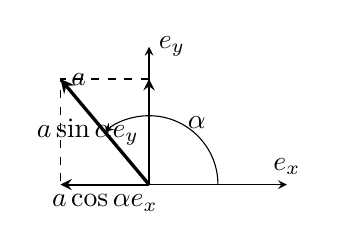
\begin{tikzpicture}
    \tikzstyle{fleche}=[->,>=stealth];
    \draw [fleche] (0,0) -- (\longueurVecteurs,0) node [above] {$\Vec{e_x}$};
    \draw [fleche] (0,0) -- (0,\longueurVecteurs) node [right] {$\Vec{e_y}$};
    \draw [fleche, very thick,\JRLblue] (0,0) -- (\angle:\longueurVecteurs) node [right] {$\Vec{a}$};
    \draw [fleche] (\longueurVecteurs/2,0) arc (0:\angle:\longueurVecteurs/2) node [midway,right] {$\alpha$};
    \draw[fleche,thick]  (0,0)--(0:{\longueurVecteurs*cos(\angle)})node[below,midway]{$a\cos\alpha\Vec{e_x}$};
     \draw[fleche,thick]  (0,0)--(90:{\longueurVecteurs*sin(\angle)})node[left,midway]{$a\sin\alpha\Vec{e_y}$};
     \draw[dashed](90:{\longueurVecteurs*sin(\angle)})-|(0:{\longueurVecteurs*cos(\angle)});
  \end{tikzpicture}
  \end{center}
  % --------------------------------------------------------- %
  \finalisationDuPartageDePage %
  % --------------------------------------------------------- %

  \end{corrige}

  % ************************************** %



  % ^^^^^^^^^^^^^^^^^^^^^^^^^^^^^^^^^^^^^^ %
  %               Question                 %
  % ^^^^^^^^^^^^^^^^^^^^^^^^^^^^^^^^^^^^^^ %
  \begin{enonce}
  	$\Vec{b}$
  \end{enonce}

  % \reponse{$b \sin(\alpha)\Vec{e_x} + b \cos (\alpha) \Vec{e_y}$}

   \begin{corrige}

  \pourcentageDeLaPartieAGauche   {0.55}
  % -------------------- Partie à gauche -------------------- %
   \initialisationPartieGauche %

  La composante suivant $\Vec{e_x}$ vaut
  \[
  b_x=\Vec{b}\cdot \Vec{e_x}=b\cos(\pi/2-\alpha)=b\sin(\alpha).
  \]
  De même, la composante suivant $\Vec{e_y}$ vaut
  \[
  b_y=\Vec{b}\cdot \Vec{e_y}=b\cos(\alpha).
  \]
  On trouve donc 
  \eqbox{
  \Vec{b} = b \sin(\alpha)\ex + b \cos (\alpha) \ey.
  }
  % --------------------------------------------------------- %
  % -------------------- Partie à droite ----------------- %
   \initialisationPartieDroite %
  \begin{center}
  		%\subimport{_images/}{projection_1_cor_b_JRL_v1.tex}
  		\def\longueurVecteurs{1.75}
  \def\angle{60}
  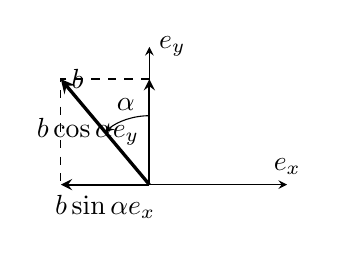
\begin{tikzpicture}
    \tikzstyle{fleche}=[->,>=stealth];
    \draw [fleche] (0,0) -- (\longueurVecteurs,0) node [above] {$\Vec{e_x}$};
    \draw [fleche] (0,0) -- (0,\longueurVecteurs) node [right] {$\Vec{e_y}$};
    \draw [fleche, very thick,\JRLblue] (0,0) -- (\angle:\longueurVecteurs) node [right] {$\Vec{b}$};
    \draw [fleche] (90:.5*\longueurVecteurs) arc (90:\angle:\longueurVecteurs/2) node [midway,above] {$\alpha$};
    \draw[fleche,thick]  (0,0)--(0:{\longueurVecteurs*cos(\angle)})node[below,midway]{$b\sin\alpha\Vec{e_x}$};
     \draw[fleche,thick]  (0,0)--(90:{\longueurVecteurs*sin(\angle)})node[left,midway]{$b\cos\alpha\Vec{e_y}$};
     \draw[dashed](90:{\longueurVecteurs*sin(\angle)})-|(0:{\longueurVecteurs*cos(\angle)});
  \end{tikzpicture}

  \end{center}
  % --------------------------------------------------------- %
  \finalisationDuPartageDePage %

  \end{corrige}

  % ************************************** %



  % ^^^^^^^^^^^^^^^^^^^^^^^^^^^^^^^^^^^^^^ %
  %               Question                 %
  % ^^^^^^^^^^^^^^^^^^^^^^^^^^^^^^^^^^^^^^ %
  \begin{enonce}
  	$\Vec{c}$
  \end{enonce}

  % \reponse{$c \cos(\alpha)\Vec{e_x} - c \sin (\alpha) \Vec{e_y}$}

  \begin{corrigeNewpage}

  \pourcentageDeLaPartieAGauche   {0.55}
  % -------------------- Partie à gauche -------------------- %
   \initialisationPartieGauche %


  On a
  \[
  c_x=\Vec{c}\cdot \Vec{e_x}=c\cos(\alpha)
  \]
  et
  \[
  c_y=\Vec{c}\cdot \Vec{e_y}=c\cos(\pi/2+\alpha)=-c\sin(\alpha).
  \]
  On retrouve ces projections à l'aide de la construction ci-contre. On a donc 
  \eqbox{
  \Vec{c} = c \cos(\alpha)\ex - c \sin (\alpha) \ey.
  }
  % --------------------------------------------------------- %
  % -------------------- Partie à droite ----------------- %
   \initialisationPartieDroite %
  \begin{center}
  	%\subimport{_images/}{projection_1_cor_c_JRL_v1.tex}
  	\def\longueurVecteurs{1.75}
  \def\angle{-30}
  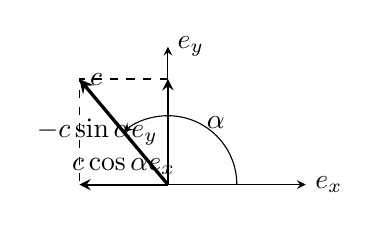
\begin{tikzpicture}
    \tikzstyle{fleche}=[->,>=stealth];
    \draw [fleche] (0,0) -- (\longueurVecteurs,0) node [right] {$\Vec{e_x}$};
    \draw [fleche] (0,0) -- (0,\longueurVecteurs) node [right] {$\Vec{e_y}$};
    \draw [fleche, very thick,\JRLblue] (0,0) -- (\angle:\longueurVecteurs) node [right] {$\Vec{c}$};
    \draw [fleche] (\longueurVecteurs/2,0) arc (0:\angle:\longueurVecteurs/2) node [midway,right] {$\alpha$};
    \draw[fleche,thick]  (0,0)--(0:{\longueurVecteurs*cos(\angle)})node[above,midway]{$c\cos\alpha\Vec{e_x}$};
     \draw[fleche,thick]  (0,0)--(90:{\longueurVecteurs*sin(\angle)})node[left,midway]{$-c\sin\alpha\Vec{e_y}$};
     \draw[dashed](90:{\longueurVecteurs*sin(\angle)})-|(0:{\longueurVecteurs*cos(\angle)});
  \end{tikzpicture}

  \end{center}
  % --------------------------------------------------------- %
  \finalisationDuPartageDePage %

  \end{corrigeNewpage}

  % ************************************** %



  % ^^^^^^^^^^^^^^^^^^^^^^^^^^^^^^^^^^^^^^ %
  %               Question                 %
  % ^^^^^^^^^^^^^^^^^^^^^^^^^^^^^^^^^^^^^^ %
  \begin{enonce}
  	$\Vec{d}$
  \end{enonce}

  % \reponse{$- d \sin(\alpha)\Vec{e_x} + d \cos (\alpha) \Vec{e_y}$}

  \begin{corrige}

  \pourcentageDeLaPartieAGauche   {0.55}
  % -------------------- Partie à gauche -------------------- %
   \initialisationPartieGauche %

  On trouve
  \[
  d_x=\Vec{d}\cdot \Vec{e_x}=d\cos(\pi/2+\alpha)=-d\sin(\alpha)
  \]
  et
  \[
  d_y=\Vec{d}\cdot \Vec{e_y}=d\cos(\alpha).
  \]
  La construction ci-contre confirme ces projections. On a donc 
  \eqbox{
  \Vec{d} = - d \sin(\alpha)\ex + d \cos (\alpha) \ey.
  }
  % --------------------------------------------------------- %
  % -------------------- Partie à droite ----------------- %
   \initialisationPartieDroite %
  \begin{center}
  	%\subimport{_images/}{projection_1_cor_d_JRL_v1.tex}
  	\def\longueurVecteurs{1.75}
  \def\angle{130}
  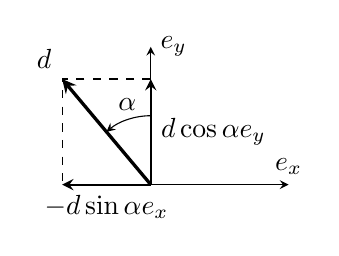
\begin{tikzpicture}
    \tikzstyle{fleche}=[->,>=stealth];
    \draw [fleche] (0,0) -- (\longueurVecteurs,0) node [above] {$\Vec{e_x}$};
    \draw [fleche] (0,0) -- (0,\longueurVecteurs) node [right] {$\Vec{e_y}$};
    \draw [fleche, very thick,\JRLblue] (0,0) -- (\angle:\longueurVecteurs) node [above left] {$\Vec{d}$};
    \draw [fleche] (90:\longueurVecteurs/2) arc (90:\angle:\longueurVecteurs/2) node [midway,above] {$\alpha$};
    \draw[fleche,thick]  (0,0)--(0:{\longueurVecteurs*cos(\angle)})node[below,midway]{$-d\sin\alpha\Vec{e_x}$};
     \draw[fleche,thick]  (0,0)--(90:{\longueurVecteurs*sin(\angle)})node[right,midway]{$d\cos\alpha\Vec{e_y}$};
     \draw[dashed](90:{\longueurVecteurs*sin(\angle)})-|(0:{\longueurVecteurs*cos(\angle)});
  \end{tikzpicture}

  \end{center}
  % --------------------------------------------------------- %
  \finalisationDuPartageDePage %

  \end{corrige}
  % *******************
\end{exo}
%%%%%%%%%%%%%%%%%%%%%%%%%%%%%%%%%%%

% %%%%%%%%%%%%%%%%%%%%%%%%%%%%%%%%%%%
% \begin{exo}[PC][1][appli]{Mouvement en spirale}
%   \hauteurLargeurCadreReponse		{8mm}{4cm}
%   Un point matériel $M(t)$ décrit une trajectoire en forme de spirale logarithmique.
%   Dans le repère polaire $(\ptO, \Vec{e_r}, \Vec{e_\theta})$, les coordonnées du point $M(t)$ sont :
%   $$
%   \begin{cases}
%   	r(t) = r_0\, e^{-t/\tau}\\
%   	\theta(t)  = \omega t
%   \end{cases}
%   $$
%   où le rayon initial $r_0$,  le temps caractéristique $\tau$ et la pulsation $\omega$ sont des constantes positives.

%   % =============================================================================== %
%   \begin{enonce}
%   	Rappeler l'expression de la vitesse $\Vec{v}(M)$ en coordonnées polaires. La calculer.
%      % \minusMedskip
%   	% {\itshape On pourra utiliser la formule donnée dans l'entraînement précédent}
%   \end{enonce}

%   \reponse{$r_0e^{-t/\tau}\left(-\frac{1}{\tau}\Vec{e_r}+\omega\Vec{e_\theta} \right)$}

%   \begin{corrige}
%   	On a $ \Vec{v}(M)=\dot{r} \Vec{e_r}+ r\dot{\theta}\Vec{e_\theta}=r_0 e^{-t/\tau}\left(-\frac{1}{\tau}\Vec{e_r}+\omega\Vec{e_\theta} \right)$.
%   \end{corrige}
%   % ************************************** %

%   % =============================================================================== %
%   \begin{enonce}
%     L'accélération en coordonnées polaires s'écrit :
%   $$
%   \Vec{a}(M)=\left(\ddot{r}-r\dot{\theta}^2\right) \Vec{e_r}+\left(2\dot{r}\dot{\theta}+r\ddot{\theta}\right) \Vec{e_\theta}.
%   $$
%   	Déterminer l'expression de l'accélération $\Vec{a}(M)$.
%   \end{enonce}

%   \reponse{$r_0 e^{-t/\tau}  \left(\left(\frac{1}{\tau^2}-\omega^2\right)\Vec{e_r}-\left(2\frac{\omega}{\tau}\right)\Vec{e_\theta}\right)$}

%   \begin{corrige}
%   	On a $\Vec{a}(M)=r_0 e^{-t/\tau}  \left(\left(\frac{1}{\tau^2}-\omega^2\right)\Vec{e_r}-\left(2\frac{\omega}{\tau}\right)\Vec{e_\theta}\right)$.
%   \end{corrige}
%   % ************************************** %
%   On donne les valeurs suivantes :
%   $\omega=\SI{4,78}{tour.min^{-1}}$,  $\tau=\SI{2,0}{s}$ et $r_0=\SI{4,0}{cm}$.

%   % =============================================================================== %
%   \begin{enonce}
%   	Dans ces conditions, l'accélération est-elle radiale ou orthoradiale ?
%   \end{enonce}

%   \reponse{orthoradiale}

%   \begin{corrige}
%   	On a $\omega=\SI{4,78}{tour.min^{-1}}=\frac{\num{4,78}\times 2\pi\ \si{rad}}{\SI{60}{s}}=\SI{0,5}{rad.s^{-1}}$ et
%   	$\frac{1}{\tau^2}-\omega^2=\left(\frac{1}{\num{0,5}^2}-\omega^2 \right)=\SI{0}{s^{-2}}$.

%   	Ainsi, on a
%   	$\Vec{a}(M,t)=-2r_0 e^{-t/\tau} \Vec{e_\theta}$.	L'accélération est donc orthoradiale.
%   \end{corrige}
%   % ************************************** %
%   \begin{enonce}
%   	Le mouvement de $M$ est-il accéléré ou décéléré ?
%   \end{enonce}

%   \reponse{décéléré}

%   \begin{corrige}
%   	On a $\Vec{a}(M,t)\cdot \Vec{e_\theta} =-2r_0 e^{-t/\tau} <0$.
%   	Le mouvement est donc décéléré.
%   \end{corrige}
%   % ************************************** %
%   \hauteurLargeurCadreReponse		{8mm}{6cm}

%   \begin{enonce}
%   	Déterminer alors l'équation polaire de la trajectoire de $M$.
%   \end{enonce}

%   \reponse{$r = r_0e^{-\theta}$}

%   \begin{corrige}
%   	On a $r = r_0e^{-t/\tau}$ et $t=\frac{\theta}{\omega}$. Donc, on a
%   	$r = r_0e^{-\theta/(\omega\times \tau)} = r_0e^{-\theta}$ car $\omega \tau = 1$.
%   \end{corrige}
% \end{exo}
% %%%%%%%%%%%%%%%%%%%%%%%%%%%%%%%%%%%


%%%%%%%%%%%%%%%%%%%%%%%%%%%%%%%%%%%
\begin{exo}[PC][2][TD]{La spirale logarithmique}
  \Notions{\item Coordonnées polaires \task Vitesse \task Accélération}
  Un point ${\rm M}(t)$ décrit une trajectoire en forme de spirale dans un référentiel $\Rcal$.
  Dans le repère polaire $(\ptO, \Vec{e_r}, \Vec{e_\theta})$, les coordonnées du point ${\rm M}(t)$ sont :
  \begin{equation}
    \begin{cases}
      r(t) = r_0\, e^{-t/\tau},\\
      \theta(t)  = \omega t,
    \end{cases}
  \end{equation}
  où $r_0$, $\tau$ et $\omega$ sont des constantes positives.

  \begin{quest}
    \question {
  	Déterminer la vitesse $\Vec{v}(M)$ en coordonnées polaires.
    } \sol{
      	On a $ \Vec{v}(M)=\dot{r} \Vec{e_r}+ r\dot{\theta}\Vec{e_\theta}$, avec $\dot{\theta} = \omega$ et $\dot{r} = -\frac{r_0}{\tau}e^{-t/\tau}$, d'où l'on tire 
        \eqbox{
       \Vec{v}(M)   = \frac{r_0}{\tau} e^{-t/\tau}\left(-\Vec{e_r}+\omega\tau\Vec{e_\theta} \right).
          }
    }

  \end{quest}
  L'accélération en coordonnées polaires s'écrit :
  % $$
  \begin{equation}
    \Vec{a}(M)=\left(\ddot{r}-r\dot{\theta}^2\right) \Vec{e_r}+\left(2\dot{r}\dot{\theta}+r\ddot{\theta}\right) \Vec{e_\theta}.
  \end{equation}
  % $$
\begin{quest}
  \question {
  	Déterminer l'accélération $\Vec{a}(M)$.
} \sol{
  On calcule les dérivées de $r$ et $\theta$ par rapport au temps :
  $$
  \ddot{r} = \frac{r_0}{\tau^2}e^{-t/\tau} \quad \text{et} \quad \ddot{\theta} = 0.
  $$ç
  Ainsi l'accélération s'écrit 
  \eqbox{
  \Vec{a}(M)= \frac{r_0}{\tau^2} e^{-t/\tau}  \left[\left(1-\omega^2\tau^2\right)\Vec{e_r}-2\omega \tau\Vec{e_\theta}\right].
  }
  	% On a $\Vec{a}(M)=r_0 e^{-t/\tau}  \left(\left(\frac{1}{\tau^2}-\omega^2\right)\Vec{e_r}-\left(2\frac{\omega}{\tau}\right)\Vec{e_\theta}\right)$.
}
\end{quest}
  On donne les valeurs suivantes :
  $\omega=\SI{4,78}{tour.min^{-1}}$,  $\tau=\SI{2,0}{s}$ et $r_0=\SI{4,0}{cm}$.

  \begin{quest}
    \question {
  	Dans ces conditions, l'accélération est-elle radiale ou orthoradiale ?
} \sol{
  	On a $\omega=\SI{4,78}{tour.min^{-1}}=\frac{\num{4,78}\times 2\pi\ \si{rad}}{\SI{60}{s}}=\SI{0,5}{rad.s^{-1}}$ et donc
  	$1-\omega^2\tau^2=\SI{0}{}$.

  	Ainsi, l'accélération est \fbox{orthoradiale}, d'expression
    \eqbox{
      \Vec{a}(M,t)= -a_0 e^{-t/\tau} \Vec{e_\theta},
      }
      avec $a_0 = \frac{2r_0\omega}{\tau}  = \SI{4}{cm.s^{-2}}$.
}
\question {
  	Le mouvement de $\rm M$ est-il accéléré ou décéléré ?
} \sol{
  	La composante orthoradiale de l'accélération vaut $a_\theta = \Vec{a}(M,t)\cdot \Vec{e_\theta} =-a_0 e^{-t/\tau} <0$.
  	Le mouvement est donc \fbox{décéléré}.
}
\question {
  	Déterminer l'équation polaire de la trajectoire de $M$.
} \sol{
  L'équation polaire est la donnée de la fonction $r(\theta)$. Il faut donc exprimer la fonctiom $t(\theta)$ puis remplacer dans l'expression de $r(t)$. On a 
  	 $t=\frac{\theta}{\omega}$ et $r = r_0e^{-t/\tau}$, soit 
  	$r = r_0e^{-\theta/(\omega\times \tau)}$. Or $\omega \tau = 1$ dans notre exemple, et donc 
    \eqbox{
      r(\theta) = r_0e^{-\theta},
    }
    avec $r_0 = \SI{4}{cm}$. Au bout d'un tour, le rayon est divisé par $e^{-2\pi} \simeq \num{0,0018}$.
}
\end{quest}
\end{exo}
%%%%%%%%%%%%%%%%%%%%%%%%%%%%%%%%%%%


%%%%%%%%%%%%%%%%%%%%%%
\begin{exo}[PCSI][1][colle]{Bretelle d’autoroute}
Un conducteur, au volant de son automobile, que  l'on assimilera a un point matériel, se déplace sur l'autoroute à la vitesse $V_0=\SI{110}{km/h}$. Il souhaite sortir de l'autoroute en utilisant une bretelle de sortie assimilée à un arc de cercle plan horizontal de rayon $R=\SI{50}{m}$.

Pour éviter de déraper dans la bretelle, la norme de l'accélération du véhicule doit rester inférieure à $a_m=\SI{10}{m.s^{-2}}$ à tout instant.
\begin{quest}
\QR{
Montrez que la voiture ne peut pas prendre la bretelle à la vitesse $V_0$ sans risquer de quitter la route.
}{
On a d'après le cours $||a|| = \frac{V_0^2}{R} \approx 22 > \SI{10}{m.s^{-2}}$. La voiture va donc déraper puis quitter la route
}


\QR{
Montrez que si l'on entre dans la bretelle à la vitesse $V_0$ et qu'on freine dans le virage, alors cela augmente le risque de sortir de la route.
}{
On a ici une accélération radiale donc suivant $\er$, l'ajout d'une accélération orthoradiale va donc augmenter la norme du vecteur accélération et donc augmenter le risque de dérapage.
}


\QR{
Calculez la vitesse maximale à laquelle la voiture peut décrire le virage sans risque de dérapage.
}{
$\frac{V_0^2}{R} = a_m \Rightarrow V_0 = \sqrt{R a_m} \approx \SI{80,5}{km.h^{-1}}$
}
\end{quest}
\end{exo}
%%%%%%%%%%%%%%%%%%%%%%%%%%%%%

%%%%%%%%%%%%%%%%%%%%%%%%%%%%%%%%%%%%%%%%%%%%%%%%%%%%%%%%%%%%%%%%
\begin{exo}[PCSI][2][colle]{Course automobile}
Deux pilotes s'élancent sur une ligne droite. Le premier démarre à $t=0$ avec une accélération constante de $\SI{4}{m.s^{-2}}$ alors que le deuxième, ayant une meilleure voiture mais de moins bons réflexes, démarre à $t=\SI{1}{s}$ avec une accélération constante \SI{5}{m.s^{-2}}.
\begin{quest}
\question { Déterminer la durée qu'il faut au second pilote pour rattraper le premier, et la distance minimale de route qu'il faut pour qu'il puisse le doubler.
}
\question { Déterminer les vitesses à l'instant du dépassement.}
\end{quest}
\end{exo}
%%%%%%%%%%%%%%%%%%%%%%%%%%%%%%%%%%%%%%%%%%%%%%%%%%%%%%%%%%%%%%%%

%%%%%%%%%%%%%%%%%%%%%%%%%%%%%%%%%%%%%%%%%%%%%%%%%%%%%%%%%%%%%%%%
\begin{exo}[PCSI]{Éléments cinématiques en coordonnées cylindriques}
On considère un point $M$ en mouvement dont les coordonnées cylindriques sont $r(t)=a_{0}t^2+r_0$, $\theta(t)=\omega t-\theta_0$ et $z(t)=-vt$ avec $r_0=\SI{1}{m}$, $a_0=\SI{1}{m.s^{-2}}$, $\omega=\SI{3}{rad.s^{-1}}$, $\theta_0=\SI{2}{rad}$ et $v=\SI{2}{m.s^{-1}}$.
\begin{quest}
\question { Rappeler les expressions des vecteurs de la base cylindrique dans la base cartésienne, et utiliser ces expressions pour retrouver les expressions générales des vecteurs vitesse et accélération dans la base cylindrique.}
\question { Calculer ensuite la norme de la vitesse du point $M$ à l'instant $t=\SI{1}{s}$, puis son accélération à l'instant initial ($t=0$).}
\end{quest}
\end{exo}
%%%%%%%%%%%%%%%%%%%%%%%%%%%%%%%%%%%%%%%%%%%%%%%%%%%%%%%%%%%%%%%%

%%%%%%%%%%%%%%%%%%%%%%%%%%%%%%%%%%%%%%%%%%%%%%%%%%%%%%%%%%%%%%%%
\begin{exo}[PCSI][2][colle]{Une course de voitures télécommandées}
Deux enfants font une course de voitures télécommandées. Ils ont le choix entre deux voitures: la rouge, qui accélère à \SI{2}{m.s^{-2}} et possède une vitesse maximale de \SI{12}{km.h^{-1}}; et la bleue, qui accélère à \SI{3}{m.s^{-2}} mais dont la vitesse maximale n'est que de \SI{10}{km.h^{-1}}.
\begin{quest}
\question { Sur une distance de \SI{15}{m}, quelle est la voiture qui remporte la course si elles partent en même temps ?
} \sol{
Notons $a_{i}$ l'accélération de la voiture $i$= rouge,bleue, et $v_i$ la vitesse maximale de la voiture $i$. Pour chaque voiture, on peut exprimer la loi horaire de la $1$ere phase du mouvement comme
$$
\dd{v}{t} = a_i \Rar v(t) = a_i t \Rar x(t)=a_i \frac{t^2}{2}.
$$
En effet, les conditions initiales ont : vitesse nulle, abscisse nulle. Cette $1$ere phase du mouvement finit lorsque la voiture atteint la vitesse maximale $v_i$, soit lorsque
$$
v(t)= v_i = a_i t \Rar t = t_i = \frac{v_i}{a_i} = \begin{cases}
\SI{1.7}{s}& \text{ pour la rouge} \\
\SI{0.9}{s} & \text{ pour la bleue}.
\end{cases}
$$
La loi horaire de la $2$eme phase du mouvement s'écrit alors
$$
x(t) = v_i(t-t_i) + a_i \frac{t_i^2}{2} = v_i t - \frac{v_i^2}{a_i} + \frac{1}{2}\frac{v_i^2}{a_i} = v_i t -\frac{1}{2}\frac{v_i^2}{a_i},
$$
où $x_i=a_i \frac{t_i^2}{2}$ représente effectivement la position de la voiture au moment où elle atteint la vitesse maximale. La voiture rouge dépasse la bleue lorsque
$$
v_1 t -\frac{1}{2}\frac{v_1^2}{a_1} = v_2 t -\frac{1}{2}\frac{v_2^2}{a_2},
$$
Soit
\eqbox{
t = \frac{1}{2(v_2-v_1)}\left(\frac{v_2^2}{a_2} - \frac{v_1^2}{a_1}\right).
}
On peut ensuite déterminer la distance $x(t)$ correspondante et la comparer à $d=\SI{15}{m}$.
}
\question { En tant que parent, déterminer la distance optimale pour que la course soit juste et ne dépende que du temps de réaction des enfants et pas des performances intrinsèques des voitures.
}
\end{quest}
\end{exo}
%%%%%%%%%%%%%%%%%%%%%%%%%%%%%%%%%%%%%%%%%%%%%%%%%%%%%%%%%%%%%%%%

%%%%%%%%%%%%%%%%%%%%%%%%%%%%%%%%%%%%%%%%%%%%%%%%%%%%%%%%%%%%%%%%
\begin{exo}[MPII]{Parcours d’un cycliste sur un vélodrome}
On s’intéresse à un cycliste, considéré comme un point matériel $M$, qui s’entraîne sur un
vélodrome constitué de deux demi-cercles reliées par deux lignes droites (figure ci-dessous).
Données : $L = \SI{62}{m}$ et $R = \SI{20}{m}$. Le cycliste part de $D$ avec une vitesse nulle dans le référentiel $\Rcal$ de la piste.

%%% FIGURE %%%
%\begin{figure}[h!]
%\centering
\begin{center}

\includegraphics[width=0.5\textwidth]{cycliste.png}
\end{center}
%%\label{fig:}
%\end{figure}
%%%%%%%%%%%

\begin{quest}
\question {  Il exerce un effort constant ce qui se traduit par une accélération constante $a$ jusqu’à l’entrée $E_1$ du premier virage. Calculer le temps $t_{E1}$ de passage en $E_1$ ainsi que la vitesse $v_{E1}$ en fonction de $a$ et $L$.
} \sol{
Le mouvement est rectiligne uniformément accéléré donc $L/2 = a\,t_{E1}^2/2$, d’où $t_{E1}=\sqrt{L/a}$ et $v_{E1} = a\,t_{E1} = \sqrt{a L}$.
}


\question { Dans le premier virage, le cycliste a une accélération tangentielle (suivant $\et$) constante
égale à $a$. Déterminer le temps $t_{S1}$ de passage en $S_1$ ainsi que la vitesse $v_{S1}$ en fonction de $a$, $L$
et $R$.


} \sol{
Le mouvement est circulaire uniformément accéléré.

Méthode 1 : l’accélération en coordonnées polaires s’écrit
$$
\Vec{a} = -r \dot{\theta}^2 \er + R\ddot{\theta} \et.
$$
L’accélération tangentielle $a=R\ddot{\theta}$ est constante. On peut ensuite intégrer $\ddot{\theta}(t)$ pour obtenir $\theta(t)$, mais c’est fastidieux.

Méthode 2 : on « déplie » la trajectoire. La distance parcourue au bout du temps $t_{S1}$ est $L/2 + \pi R = a t_{S1}^2/2$, et donc $t_{S1}=\sqrt{(2\pi R + L)/a}$ et $v_{S1} = \sqrt{(2\pi R + L) a}$.
}


\question { De même, déterminer le temps de passage après un tour $t_D$, ainsi que la vitesse
correspondante.


} \sol{
On a $t_D = \sqrt{(4\pi R + 4L)/a}$ et $v_{D} = \sqrt{(4\pi R + 4L)a}$.
}

\question { %La course s’effectue sur quatre tours ($\SI{1}{km}$).
Le tour a été effectué en $t_D = \SI{18,155}{s}$ par le britannique Chris Hoy aux Championnats du monde de 200. Déterminer la valeur de l’accélération $a$ ainsi que la vitesse atteinte en $D$. La vitesse mesurée sur piste est d’environ $\SI{60}{km.h^{-1}}$ ; que doit-on modifier dans le
modèle pour se rapprocher de la réalité ?
} 
\sol{
On trouve $a = (4\pi R + 4L)/t_D^2 = \SI{1.51}{m.s^{-2}}$ et $v_D = \SI{27.5}{m.s^{-1}} = \SI{99}{km.h^{-1}}$. En réalité, l’accélération n’est pas constante mais diminue au fur et à mesure que la vitesse augmente.
}

\end{quest}
\end{exo}
%%%%%%%%%%%%%%%%%%%%%%%%%%%%%%%%%%%%%%%%%%%%%%%%%%%%%%%%%%%%%%%%

%%%%%%%%%%%%%%%%%%%%%%%%%%%%%%%%%%%%%%%%%
\begin{exo}[MPSI][3][colle]{Poursuite du chien et du lapin}
Un lapin initialement à l'origine court à vitesse constante $w$ dans la direction des $y$ croissants. Un chien initialement à la position $x=a$, $y=0$ poursuit le lapin à vitesse constante $v$. Le vecteur vitesse du chien $\Vec{v}$ pointe à tout instant en direction du lapin.

\begin{quest}
\question { Faire un schéma du problème et représenter l'allure attendue de la trajectoire. Que se passe-t-il si $v<w$ ? $v>w$ ?}

\question { Soit $y(x)$ l'équation de la trajectoire du chien. Par des considérations géométriques, montrer que
\begin{equation}
\dfrac{\d y}{\d x} = \dfrac{y-wt}{x}.
\end{equation}
En déduire que
\begin{equation}
x \dfrac{\d^2 y}{\d x^2} = -w \dfrac{\d t}{\d x}.
\end{equation}

} \sol{
Géométrie. On a ensuite $xy'-y=-wt$ donc en dérivant $xy''=-w\d t/\d x$.
}

\question { On introduit l'abscisse curviligne $s$. Relier la norme de la vitesse $v$ à une dérivée de $s$. On pose $p=\dfrac{\d y}{\d x}$ et $k=w/v$ la vitesse relative du lapin. En déduire que
\begin{equation}
\dfrac{\d p}{\sqrt{1+p^2}} = -k \dfrac{\d x}{x}.
\end{equation}

} \sol{
On a
$$
\dfrac{\d t}{\d x} = \dfrac{\d t}{\d s} \dfrac{\d s}{\d x} = \dfrac{1}{v} \sqrt{1+y'^2}.
$$
Donc $$
xy'' = -k\sqrt{1+y'^2}.
$$
}


\question { Intégrer l'équation ci-dessus et utiliser les conditions initiales pour trouver l'équation de la trajectoire $y(x)$ dans le cas $v=w$. On indique qu'une primitive de $1/\sqrt{1+p^2}$ est la fonction $\text{argsh}(p)$, de réciproque
\begin{equation}
\text{sh}(p) = \dfrac{e^p-e^{-p}}{2}.
\end{equation}

} \sol{
L'équation s'intègre en
$$
\ln(p+\sqrt{1+p^2}) = -k\ln(x/c).
$$
soit
$$
p = \dfrac{1}{2} \left[ \left( \dfrac{x}{a}\right)^{-k} -  \left( \dfrac{a}{x}\right)^{-k} \right]
$$
Pour $k=1$ on trouve
$$
p =  -\dfrac{1}{2} \left[ \dfrac{x}{a} -   \dfrac{a}{x} \right] \Rightarrow y = -\dfrac{x^2}{4a} + \dfrac{a}{2}\left(\ln(x)-\ln(a)+\dfrac{1}{2}\right).
$$
}

\end{quest}
\end{exo}
%%%%%%%%%%%%%%%%%%%%%%%%%%%%%%%%%%%%%%
%
% %%%%%%%%%%%%%%%%%%%%%%%%%%%%%%%%%%%%%%%%%%%%%%%%%%%%%%%%%%%%%%%%
% \begin{exo}[MPII]{Parcours d’un cycliste sur un vélodrome}
% On s’intéresse à un cycliste, considéré comme un point matériel $M$, qui s’entraîne sur un
% vélodrome constitué de deux demi-cercles reliées par deux lignes droites (figure ci-dessous).
% Données : $L = \SI{62}{m}$ et $R = \SI{20}{m}$. Le cycliste part de $D$ avec une vitesse nulle dans le référentiel $\Rcal$ de la piste.
%
% %%% FIGURE %%%
% %\begin{figure}[h!]
% %\centering
% \begin{center}
% 
\includegraphics[width=0.5\textwidth]{cycliste.png}
% \end{center}
% %%\label{fig:}
% %\end{figure}
% %%%%%%%%%%%
%
% \begin{quest}
% \question {  Il exerce un effort constant ce qui se traduit par une accélération constante $a$ jusqu’à l’entrée $E_1$ du premier virage. Calculer le temps $t_{E1}$ de passage en $E_1$ ainsi que la vitesse $v_{E1}$ en fonction de $a$ et $L$.
%
%
% } \sol{
% Le mouvement est rectiligne uniformément accéléré donc $L/2 = a\,t_{E1}^2/2$, d’où $t_{E1}=\sqrt{L/a}$ et $v_{E1} = a\,t_{E1} = \sqrt{a L}$.
% }
%
%
% \question { Dans le premier virage, le cycliste a une accélération tangentielle (suivant $\et$) constante
% égale à $a$. Déterminer le temps $t_{S1}$ de passage en $S_1$ ainsi que la vitesse $v_{S1}$ en fonction de $a$, $L$
% et $R$.
%
%
% } \sol{
% Le mouvement est circulaire uniformément accéléré.
%
% Méthode 1 : l’accélération en coordonnées polaires s’écrit
% $$
% \Vec{a} = -r \dot{\theta}^2 \er + R\ddot{\theta} \et.
% $$
% L’accélération tangentielle $a=R\ddot{\theta}$ est constante. On peut ensuite intégrer $\ddot{\theta}(t)$ pour obtenir $\theta(t)$, mais c’est fastidieux.
%
% Méthode 2 : on « déplie » la trajectoire. La distance parcourue au bout du temps $t_{S1}$ est $L/2 + \pi R = a t_{S1}^2/2$, et donc $t_{S1}=\sqrt{(2\pi R + L)/a}$ et $v_{S1} = \sqrt{(2\pi R + L) a}$.
% }
%
%
% \question { De même, déterminer le temps de passage après un tour $t_D$, ainsi que la vitesse
% correspondante.
%
%
% } \sol{
% On a $t_D = \sqrt{(4\pi R + 4L)/a}$ et $v_{D} = \sqrt{(4\pi R + 4L)a}$.
% }
%
% \question { %La course s’effectue sur quatre tours ($\SI{1}{km}$).
% Le tour a été effectué en $t_D = \SI{18,155}{s}$ par le britannique Chris Hoy aux Championnats du monde de 200\question { Déterminer la valeur de l’accélération $a$ ainsi que la vitesse atteinte en $D$. La vitesse mesurée sur piste est d’environ $\SI{60}{km.h^{-1}}$ ; que doit-on modifier dans le
% modèle pour se rapprocher de la réalité ?
%
%
% } \sol{
% On trouve $a = (4\pi R + 4L)/t_D^2 = \SI{1.51}{m.s^{-2}}$ et $v_D = \SI{27.5}{m.s^{-1}} = \SI{99}{km.h^{-1}}$. En réalité, l’accélération n’est pas constante mais diminue au fur et à mesure que la vitesse augmente.
% }
%
% \end{quest}
% \end{exo}
% %%%%%%%%%%%%%%%%%%%%%%%%%%%%%%%%%%%%%%%%%%%%%%%%%%%%%%%%%%%%%%%%

